\section{Results and Discussions}
%%%%%%%%%%%%%%%%%%%%%%%%%%%%%%%%%%%%%%%%%%%%%%%%%%%%%
In this section, we are going to show some results for delamination detection in accordance with the adaptive wavenumber filtering and the FCN-DenseNet model. 
%	As we mentioned earlier, a sigmoid and a softmax functions are used at the output layer for our model, hence we have two versions of the FCN-DenseNet model with different output layer function.

The sigmoid function at the output layer of the FCN-DenseNet model computes the damage probability for each pixel, hence the damage probability ranges from (\(0 - 1\)).
Therefore, there is a need for a threshold function to exclude low probabilities of predicted damage. 
For all the following results, the threshold \(tr = 0.5\) was set, therefore any value less than \(0.5\) will be excluded from the damage map.
For the softmax function at the output layer, it computes two probabilities for each pixel: (damaged and undamaged), then an \(\argmax\) function is applied to select the highest probability between the two probabilities, therefore there is no need for thresholding. 
The FCN-DenseNet models was trained on augmented dataset up to 100 epochs, and the architecture of the FCN-DenseNet  was implemented using the open-source platform of Keras API~\cite{chollet2015keras} running on top of TensorFlow on a GeForce RTX 2080  GPU from NVIDIA.
For all scenarios, we selected a red colour to represent the detected delamination (damaged), and the blue colour to represent the healthy state (undamaged).

In the following, we are going to present three scenarios of delaminations of different locations, shapes and angles.

Figure~\ref{fig:RMS_flat_shell_Vz_438} shows the RMS of full wavefield interpolated at the bottom surface of the plate with delamination located at the top edge of the plate.
Figure~\ref{fig:m1_rand_single_delam_438} shows the ground truth image corresponding to Fig.~\ref{fig:RMS_flat_shell_Vz_438}. 
Fig.~\ref{fig:ERMSF_flat_shell_Vz_438} shows the detected delamination using the adaptive wavenumber filtering. 
The damage map represents the energy-based root mean square index of frames filtered in the wavenumber domain (ERMSF). 
It can be seen in the damage map that the delamination is detected, but still, the method boosts edge reflections which results in some noise at the edges. 
To eliminate low values from the ERMSF, a binary threshold is applied as shown in Fig.~\ref{fig:Binary_ERMSF_flat_shell_Vz_438}.
The threshold level was selected to limit the influence of edge noise and at the same time highlight the damage. 
The binary ERMSF properly indicates the location of delamination but still, there is some noise at the corners.
It results in the calculated IoU equal (\(0.10\)).
In Figs.~\ref{fig:predict_438_sigmoid_tr_0.5}, ~\ref{fig:predict_438_softmax} we present the \DIFdelbegin \DIFdel{FCN-DeneseNet }\DIFdelend \DIFaddbegin \DIFadd{FCN-DenseNet }\DIFaddend outputs with sigmoid and softmax respectively.
As shown, the FCN-DenseNet models detect the delamination without any noise at the edges as the FCN-DenseNet learned the delamination patterns from the large numerically generated dataset and can differentiate among different complex patterns such as noise.   
The IoU = \(0.73\) for sigmoid, and IoU = \(0.65\) for the softmax.
	%%%%%%%%%%%%%%%%%%%%%%%%%%%%%%%%%%%%%%%%%%%%%%%%%%%
	%first figure
	%%%%%%%%%%%%%%%%%%%%%%%%%%%%%%%%%%%%%%%%%%%%%%%%%%%
	\begin{figure} [!h]
		\centering
		\begin{subfigure}[b]{0.47\textwidth}
			\centering
			\includegraphics[scale=1]{RMS_flat_shell_Vz_438_500x500bottom.png}
			\caption{RMS bottom}
			\label{fig:RMS_flat_shell_Vz_438}
		\end{subfigure}
		\hfill
			\begin{subfigure}[b]{0.47\textwidth}
			\centering
			\includegraphics[scale=1]{m1_rand_single_delam_438.png}
			\caption{Ground truth}
			\label{fig:m1_rand_single_delam_438}
		\end{subfigure}
		\hfill
		\begin{subfigure}[b]{0.47\textwidth}
			\centering
			\includegraphics[scale=1]{ERMSF_flat_shell_Vz_438_500x500bottom.png}
			\caption{Adaptive wavenumber filtering (ERMSF)}
			\label{fig:ERMSF_flat_shell_Vz_438}
		\end{subfigure}
		\hfill
		\begin{subfigure}[b]{0.47\textwidth}
			\centering
			\includegraphics[scale=1]{Binary_ERMSF_flat_shell_Vz_438_500x500bottom.png}
			\caption{binary ERMSF}
			\label{fig:Binary_ERMSF_flat_shell_Vz_438}
		\end{subfigure}
		\hfill
		\begin{subfigure}[b]{0.47\textwidth}
			\centering
		\includegraphics[scale=1]{FCN_DenseNet_Predicted_438_sigmoid_thresholded_0.5.png}
		\caption{sigmoid \((tr = 0.5)\)}
		\label{fig:predict_438_sigmoid_tr_0.5}
		\end{subfigure}
		\hfill
		\begin{subfigure}[b]{0.47\textwidth}
			\centering
			\includegraphics[scale=1]{FCN_DenseNet_Predicted_438_softmax.png}
			\caption{softmax}
			\label{fig:predict_438_softmax}
		\end{subfigure}
		\caption{First delamination scenario based on numerical data.}
		\label{fig:RMS438}
	\end{figure} 
	%%%%%%%%%%%%%%%%%%%%%%%%%%%%%%%%%%%%%%%%%%%%%%%%%%%

In the next scenario, we present delamination located in the upper left part of the plate.
Figs.~\ref{fig:dispersion30deg_direct}, ~\ref{fig:m1_rand_single_delam_454} show the RMS of the full wavefield interpolated at the bottom surface of the plate.
Fig.~\ref{fig:ERMSF_flat_shell_Vz_454} shows the damage map obtained by using the adaptive wavenumber filtering.
The adaptive wavenumber filtering method picks some noise at the edges but the shape of delamination is clearly highlighted by high values of damage map.
Nevertheless, there is still some noise after applying threshold as it is shown in Fig.~\ref{fig:Binary_ERMSF}.
The IoU for this case is \(0.61\).
In Figs.~\ref{fig:predict_454_sigmoid_tr_0.5}, ~\ref{fig:predict_454_softmax} we present the FCN-DeneseNet outputs with sigmoid and softmax, respectively.
The sigmoid detect the delamination with IoU = \(0.58\), and for the softmax with IoU = \(0.60\).
As we can see also for this scenario, the FCN-DenseNet only detects the delamination patterns without unwanted noise.
%%%%%%%%%%%%%%%%%%%%%%%%%%%%%%%%%%%%%%%%%%%%%%%%%%%
	\begin{figure} [!h]
		\centering
		\begin{subfigure}[b]{0.47\textwidth}
			\centering
			\includegraphics[scale=1]{RMS_flat_shell_Vz_454_500x500bottom.png}
			\caption{RMS bottom}
			\label{fig:dispersion30deg_direct}
		\end{subfigure}
		\hfill
		\begin{subfigure}[b]{0.47\textwidth}
			\centering
			\includegraphics[scale=1]{m1_rand_single_delam_454.png}
			\caption{Ground truth}
			\label{fig:m1_rand_single_delam_454}
		\end{subfigure}
		\hfill
		\begin{subfigure}[b]{0.47\textwidth}
			\centering
			\includegraphics[scale=1]{ERMSF_flat_shell_Vz_454_500x500bottom.png}
			\caption{Adaptive wavenumber filtering (ERMSF)}
			\label{fig:ERMSF_flat_shell_Vz_454}
		\end{subfigure}
		\hfill
		\begin{subfigure}[b]{0.47\textwidth}
			\centering
			\includegraphics[scale=1]{Binary_ERMSF_flat_shell_Vz_454_500x500bottom.png}
			\caption{Binary ERMSF}
			\label{fig:Binary_ERMSF}
		\end{subfigure}
		\hfill
		\begin{subfigure}[b]{0.47\textwidth}
			\centering
			\includegraphics[scale=1]{FCN_DenseNet_Predicted_454_sigmoid_thresholded_0.5.png}
			\caption{sigmoid (tr =\(0.5\))}
			\label{fig:predict_454_sigmoid_tr_0.5}
		\end{subfigure}
		\hfill	
		\begin{subfigure}[b]{0.47\textwidth}
			\centering
			\includegraphics[scale=1]{FCN_DenseNet_Predicted_454_softmax.png}
			\caption{softmax}
			\label{fig:predict_454_softmax}
		\end{subfigure}
		\caption{Second delamination scenario based on numerical data.}
		\label{fig:RMS454}
	\end{figure} 
%%%%%%%%%%%%%%%%%%%%%%%%%%%%%%%%%%%%%%%%%%%%%%%%%%%	
%	Figs.[~\ref{fig:unthresholded438}, ~\ref{fig:unthresholded454}] show the original damage maps without thresholding for the FCN-DenseNet with sigmoid function for the first and second scenarios respectively. 
%	As shown from the figs, the predicted output has a range or probabilities of damage. 
%	Accordingly, we apply threshold to exclude these low damage probabilities.
%	\begin{figure} [!h] 
%		\centering
%		\begin{subfigure}[b]{0.47\textwidth}
%		\centering
%		\includegraphics[scale=1]{sigmoid_unthresholded438.png}
%		\caption{}
%		\label{fig:unthresholded438}
%		\end{subfigure}
%	\hfill	
%	\begin{subfigure}[b]{0.47\textwidth}
%		\centering 	
%		\includegraphics[scale=1]{sigmoid_unthresholded454.png}
%		\caption{}
%		\label{fig:unthresholded454}
%	\end{subfigure}
%	\caption{Unthresholded damage maps for FCN-DenseNet/sigmoid}
%	\label{fig:unthresholded}
%	\end{figure}

In Fig.~\ref{fig:RMS433} we present the third scenario where the damage map obtained by the adaptive wavenumber filtering method is useful for delamination visualisation but the FCN-DenseNet model failed.
%%%%%%%%%%%%%%%%%%%%%%%%%%%%%%%%%%%%%%%%%%%%%%%%%%%
% third figure
%%%%%%%%%%%%%%%%%%%%%%%%%%%%%%%%%%%%%%%%%%%%%%%%%%%
\begin{figure}[!h]
	\centering
	\begin{subfigure}[b]{0.47\textwidth}
		\centering
		\includegraphics[scale=1]{RMS_flat_shell_Vz_433_500x500bottom.png}
		\caption{RMS bottom}
		\label{fig:RMS_flat_shell_Vz_433}
	\end{subfigure}
	\hfill
	\begin{subfigure}[b]{0.47\textwidth}
		\centering
		\includegraphics[scale=1]{m1_rand_single_delam_433.png}
		\caption{ground truth}
		\label{fig:m1_rand_single_delam_433}
	\end{subfigure}
	\hfill
	\begin{subfigure}[b]{0.47\textwidth}
		\centering
		\includegraphics[scale=1]{ERMSF_flat_shell_Vz_433_500x500bottom.png}
		\caption{Adaptive wavenumber filtering (ERMSF)}
		\label{fig:ERMSF_flat_shell_Vz_433}
	\end{subfigure}
	\hfill
	\begin{subfigure}[b]{0.47\textwidth}
		\centering
		\includegraphics[scale=1]{Binary_ERMSF_flat_shell_Vz_433_500x500bottom.png}
		\caption{binary ERMSF}
		\label{fig:Binary_ERMSF_flat_shell_Vz_433}
	\end{subfigure}
	\caption{Third delamination scenario based on numerical data.}
	\label{fig:RMS433}
\end{figure} 

Figures.~\ref{fig:RMS_flat_shell_Vz_433}, ~\ref{fig:m1_rand_single_delam_433} show the RMS of the full wavefield interpolated at the bottom surface of the plate with delamination located at the upper left corner of the plate and its corresponding ground truth, respectively.
It is impossible to notice any changes of RMS pattern caused by the delamination (Fig.~\ref{fig:RMS_flat_shell_Vz_433}).
It should be noted that this image is fed to the FCN-DenseNet model whereas the full wavefield (all frames) are used in the adaptive wavenumber filtering method.
In extreme cases, like this, conventional signal processing has an advantage over the FCN-DenseNet model.
As shown in Fig.~\ref{fig:ERMSF_flat_shell_Vz_433} representing the damage map obtained by the adaptive wavenumber filtering technique, the delamination location can be identified by a well-trained expert. 
However, the values of the damage map corresponding to the delamination location are on the same level as the noise.
Hence, when binary thresholding is applied, only some false damage indications are highlighted near corners of the plate as show in Fig.~\ref{fig:Binary_ERMSF_flat_shell_Vz_433}. 
For this case IoU= \(0\) for all considered methods \DIFdelbegin \DIFdel{.
 }\DIFdelend \DIFaddbegin \DIFadd{including FCN-DenseNet.
FCN-DenseNet outputs are not shown because whole images are blue.
 }\DIFaddend 

Delaminations located near edges or corners are difficult to detect due to edge wave reflections which have similar patterns as delamination reflections. 
The problem arises for both conventional and deep learning techniques\DIFdelbegin \DIFdel{. 
However, to solve this issue }\DIFdelend \DIFaddbegin \DIFadd{, especially for delamination of small size. 
}

\DIFadd{It should be noted, however, that if larger delamination appear near the corner, FCN-DenseNet is able to identify it correctly.
Such situation is presented in Fig.~\ref{fig:corner_delam}.	
}

\begin{figure}[!h]
	\centering
	\begin{subfigure}[b]{0.47\textwidth}
		\centering
		\includegraphics[scale=1]{GT_385.png}
		\caption{\DIFaddFL{ground truth}}
		\label{fig:GT_385}
	\end{subfigure}
	\hfill
	\begin{subfigure}[b]{0.47\textwidth}
		\centering
		\includegraphics[scale=1]{fcn_densenet_Pred_softmax_385.png}
		\caption{\DIFaddFL{FCN-DenseNet}}
		\label{fig:FCN-DenseNet_385}
	\end{subfigure}
	\caption{\DIFaddFL{The delamination scenario with larger delamination near the corner based on numerical data.}}
	\label{fig:corner_delam}
\end{figure} 

\DIFadd{The problem with delaminations at the corners }\DIFaddend for the FCN model \DIFdelbegin \DIFdel{, we need to enhance the }\DIFdelend \DIFaddbegin \DIFadd{can be alleviated by enhancing }\DIFaddend feature extraction process by obtaining more data to train the model to recognise and learn new patterns.

In Table~\ref{tab:iou} we present the maximum, minimum and mean value of IoU for the adaptive filtering and FCN-DenseNet for sigmoid (threshold = \(0.5\)) and softmax for all testing images.
\DIFaddbegin \DIFadd{It can be concluded that the FCN-DenseNet model surpasses significantly adaptive wavenumber filtering method. 
	}\DIFaddend \begin{table}
	 \renewcommand{\arraystretch}{1.3}
		\centering
		\caption{IoU for all models}
		\label{tab:iou}
		\resizebox{\textwidth}{!}{\begin{tabular}{ccccccccccccc}
				\toprule
				&  &  &  &  &  & \multicolumn{7}{c}{FCN-Dense Model} \\ \cline{7-13} 
				&  & \multicolumn{3}{c}{Adaptive filtering} &  & \multicolumn{3}{c}{sigmoid} &  & \multicolumn{3}{c}{softmax} \\ \cline{3-5} \cline{7-9} \cline{11-13} 
				&  & min & max & mean &  & min & max & mean &  & \multicolumn{1}{c}{min} & \multicolumn{1}{c}{max} & \multicolumn{1}{c}{mean} 
				%\\ \cline{3-13} 
				\\ \cline{3-5} \cline{7-9} \cline{11-13} 
				\multicolumn{2}{c}{IoU} &0&0.648&0.373& &0&0.933&0.616&  &0&0.878&0.623\\ 
				\bottomrule
		\end{tabular}}
	\end{table}

Every single value of the IoU was estimated for all testing images using FCN-DenseNet with a sigmoid at the output layers.
It is expected that as we increase the threshold, the IoU will decrease because some of the detected output values will be excluded.
Therefore, selecting the proper threshold value is important for maximizing IoU\DIFaddbegin \DIFadd{, and this is the reason why inductive bias is important}\DIFaddend . 
Fig.~\ref{fig:iou_fcn} shows the maximum and mean IoU for all testing images depending on the threshold value. 
The IoU is decreasing along with the threshold increment in the range of (\(0-1\)).
	\begin{figure}[!h] 
		\centering
		\includegraphics[width=\textwidth]{fcn_densenet_iou.png}
		\centering
		\caption{IoU for FCN-DenseNet with sigmoid of a range of thresholds \([0-1]\)} 
		\label{fig:iou_fcn}
	\end{figure}

In Fig.~\ref{fig:Exp_ERMS_teflon}, we present an experimental scenario of CFRP with Teflon insert as artificial delamination.
Similarly to the numerical case, the frequency of \(50\) kHz was used to excite the transducer which was placed at the centre of the plate.
As shown in Fig.~\ref{fig:ERMSF_CFRP_teflon} the adaptive wavenumber filtering method is able to detect the delamination. 
Fig.~\ref{fig:Binary_ERMSF_CFRP} shows the binary thresholded output which precisely highlights the location of delamination. 
Even the shape of the delamination is quite well represented.
The IoU for this scenario was \(0.401\). 

The FCN-DenseNet model detected the delamination with both a sigmoid and softmax functions as shown in Fig.~\ref{fig:EXP_predict_sigmoid} and Fig.~\ref{fig:EXP_predict_softmax}, respectively.
The IoU for FCN-DenseNet model was \(0.053\) and \(0.081\) for a sigmoid and softmax, respectively.
These poor results of predictions are expected since we trained our model only on numerically generated data.
However, apart from the noise at the edges and at the transducer location, the FCN-DenseNet could detect the delamination in the experimentally generated image.
It means that the model has excellent generalisation capabilities and is able to detect delamination based on previously unseen data.
We expect, that the generalisation capabilities and, in turn, delamination identification performance, can be further enhanced by training the model on experimental data.
However, the generation of large dataset comprised of experiments with various defects is troublesome.
	\begin{figure} [!h]
		\centering
		\begin{subfigure}[b]{0.47\textwidth}
			\centering
			\includegraphics[scale=1]{ERMS_CFRP_teflon_3o_375_375p_50kHz_5HC_x12_15Vpp.png}
			\caption{ERMS CFRP Teflon inserted}
			\label{fig:Delamination}
		\end{subfigure}			
		\hfill
		\begin{subfigure}[b]{0.47\textwidth}
			\centering 	
			\includegraphics[scale=1]{label_CFRP_teflon_3o_375_375p_50kHz_5HC_x12_15Vpp.png}
			\caption{Ground truth} 
			\label{fig:damage_label}
		\end{subfigure}
		\hfill
		\begin{subfigure}[b]{0.47\textwidth}
			\centering
			\includegraphics[scale=1]{ERMSF_CFRP_teflon_3o_375_375p_50kHz_5HC_x12_15Vpp.png}
			\caption{ERMSF} 
			\label{fig:ERMSF_CFRP_teflon}
		\end{subfigure}
		\hfill
		\begin{subfigure}[b]{0.47\textwidth}
		\centering
		\includegraphics[scale=1]{Binary_ERMSF_CFRP_teflon_3o_375_375p_50kHz_5HC_x12_15Vpp.png}
		\caption{Binary ERMSF} 
		\label{fig:Binary_ERMSF_CFRP}
		\end{subfigure}
		\hfill
		\begin{subfigure}[b]{0.47\textwidth}
			\centering
			\includegraphics[scale=1]{Predicted_Predicted_ERMS_CFRP_teflon_3o_375_375p_50kHz_5HC_x12_15Vpp_7__threshold_0.5_sigmoid.png}
			\caption{FCN DenseNet: sigmoid \((tr = 0.5)\)} 
			\label{fig:EXP_predict_sigmoid}
		\end{subfigure}
		\hfill
		\begin{subfigure}[b]{0.47\textwidth}
			\centering
			\includegraphics[scale=1]{Predicted_Predicted_ERMS_CFRP_teflon_3o_375_375p_50kHz_5HC_x12_15Vpp_7_softmax.png}
			\caption{FCN DenseNet: softmax} 
			\label{fig:EXP_predict_softmax}
		\end{subfigure}
			\caption{Experimental results}
			\label{fig:Exp_ERMS_teflon}
		\end{figure}
%%%%%%%%%%%%%%%%%%%%%%